\section{Chainball (60pts)}
如图\ref{fig:chainball} 所示,一个简单的链条球模型由三个质量为$m$的球体和两根无质量的轻绳组成。现在固定最上方的一个球体,并自然下垂。绳子的长度均为\(l\), 重力加速度为\(g\).

\begin{figure}[htbp]
	\centering
	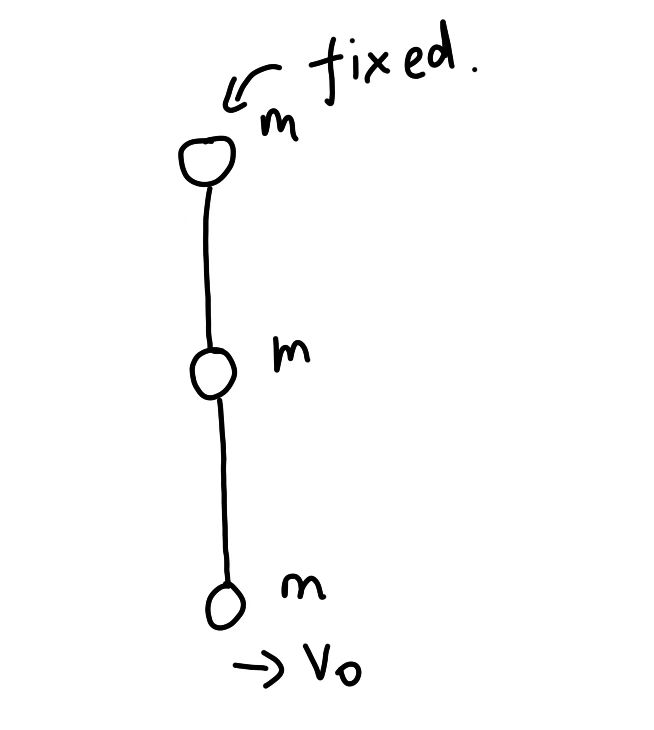
\includegraphics[width=0.3\textwidth]{chainball}
	\caption{三个质量为$m$的球体由两根无质量的轻绳连接成链条球模型,最上方的球体固定.}
	\label{fig:chainball}
\end{figure}

\begin{enumerate}
	\item 现在突然给予最下方的球体一个向右的初速度$v_0$,求出最下方球体的水平方向上的位移随时间变化的关系式。(设\(v_{0}\)很小可以视为小振动)(30pts)
	\item 在第一小问的设定下,最下方球体水平方向上最远可以达到的位移是多少?(4pts)
	\item 现在只限制下方小球的初速度为向右的初速度为\(v_0\),请问是否有方式使得摆动看起来“更有规律”?即:每次当中间球体回到最低点时,最下方的球体也回到最低点。如果有,请给出所有还需要的条件;如果没有,请给出理由。(16ps)
	\item 下面考虑一个更复杂一点的情况:现在由\(n+2\)个质量为\(m\)的球体组成类似的链条球模型。如图\ref{fig:chainball2}所示。为了更容易计算,现设定如下:初始时上方\(n\)个球均是固定的,只有最下方两个球可以自由移动,仍然给予最下方球初速度\(v_{0}\),当倒数第二个球体再次回到最低点的时刻,通过Teyvat的神秘力量使得最后一根绳子断裂(即编号为0的球体会脱落),同时解除编号为2的球体的锁定。如此递推,每次保持只有两个球体会活动,直到只剩下编号为\(n\)与\(n+1\)的球体。请求出此时编号为\(n\)的球体的水平方向上的位移随时间变化的关系式。(\(v_{0}\)仍然认为只能引起小振动)(10pts)
	\begin{figure}[htbp]
	\centering
	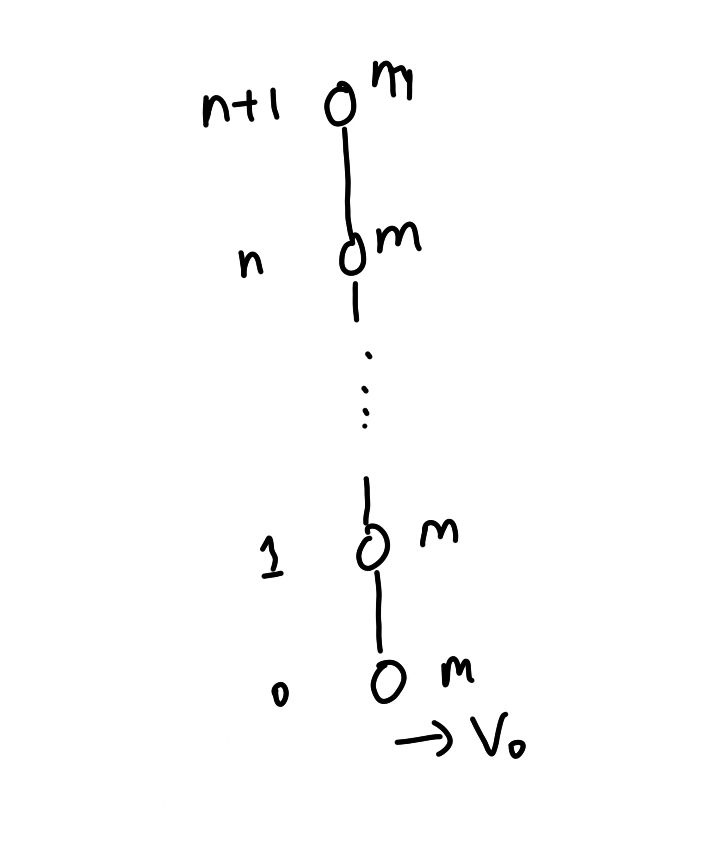
\includegraphics[width=0.3\textwidth]{chainball2}
	\caption{多级链条球.}
	\label{fig:chainball2}
 \end{figure}
\end{enumerate}

\section*{Answer 1}
\begin{enumerate}
	\item 我们设第一根绳子的向右偏离竖直方向的角度为\(\theta_1\),第二根绳子的向右偏离竖直方向的角度为\(\theta_2\),写出系统动能与势能:
	\begin{align*}
		T &= \frac{1}{2}ml^{2}\dot{\theta}_1^2 + \frac{1}{2}ml^{2}(\dot{\theta}_1+\dot{\theta}_2)^2 \\
		V &= -mglcos\theta_1 - mgl(cos\theta_1+cos\theta_2) \\
		  &= V_{0} + mgl(\theta_1^2 + \frac{1}{2}\theta_2^2) 
	\end{align*}
	进而有拉格朗日函数:
	\begin{align*}
		L &= T - V \\
		  &= \frac{1}{2}ml^{2}\dot{\theta}_1^2 + \frac{1}{2}ml^{2}(\dot{\theta}_1+\dot{\theta}_2)^2 - mgl(\theta_1^2 + \frac{1}{2}\theta_2^2) 
	\end{align*}
	对\(\theta_1\)与\(\theta_2\)分别求拉格朗日方程:
	\begin{align*}
		\frac{d}{dt}(\frac{\partial L}{\partial \dot{\theta}_1}) - \frac{\partial L}{\partial \theta_1} &= 0 \\
		\frac{d}{dt}(\frac{\partial L}{\partial \dot{\theta}_2}) - \frac{\partial L}{\partial \theta_2} &= 0 
	\end{align*}
	进而有:
	\begin{align*}
		2mgl\theta_1 + ml^{2}\ddot{\theta}_1 + ml^{2}(\ddot{\theta}_1+\ddot{\theta}_2) &= 0 \\
		mgl\theta_2 + ml^{2}(\ddot{\theta}_1+\ddot{\theta}_2) &= 0 
	\end{align*}
	进而有:
	\begin{align*}
		2\ddot{\theta}_1 + \ddot{\theta}_2 + 2\frac{g}{l}\theta_1 &= 0 \\
		\ddot{\theta}_1 + \ddot{\theta}_2 + \frac{g}{l}\theta_2 &= 0 
	\end{align*}
	令\(w_{0}^2= \frac{g}{l}\), 下面开始计算简正坐标:下式乘以\(\lambda\)加上上式可以得到:
	\begin{align*}
		(2+\lambda)\ddot{\theta}_1 + (1+\lambda)\ddot{\theta}_2 + 2w_{0}^2\theta_1 + \lambda w_{0}^2\theta_2 &= 0 
	\end{align*}
	注意到\(\lambda \neq 0 \) or \(-1\).应有:
	\begin{align*}
		\frac{2+\lambda}{1+\lambda} = \frac{2}{\lambda}
	\end{align*} 
	解的\(\lambda = \pm \sqrt{2}\),回代进而可以找到两个简正坐标:
	\begin{align*}
		q_1 &= \sqrt{2}\theta_1 + \theta_2 \\
		q_2 &= \sqrt{2}\theta_1 - \theta_2 
	\end{align*}
	使得:
	\begin{align*}
		\ddot{q}_1 + \frac{\sqrt{2}}{1+\sqrt{2}}w_{0}^2 q_1 &= 0 \\
		\ddot{q}_2 + \frac{\sqrt{2}}{-1+\sqrt{2}}w_{0}^2 q_2 &= 0 
	\end{align*}
	分别获得了两个简谐振动的频率:
	\begin{align*}
		\omega_1 &= \sqrt{2-\sqrt{2}}w_{0} \\
		\omega_2 &= \sqrt{2+\sqrt{2}}w_{0} 
	\end{align*}
	根据初始条件\(\theta_1=0\), \(\theta_2=0\), \(\dot{\theta}_1=0\), \(\dot{\theta}_2=\frac{v_0}{l}\)可以得到简正坐标的初始条件:
	\begin{align*}
		q_1(0) &= 0 \\ 
		q_2(0) &= 0 \\ 
		\dot{q}_1(0) &= \frac{v_0}{l} \\ 
		\dot{q}_2(0) &= -\frac{v_0}{l} 
	\end{align*}
	进而可以得到简正坐标的解:
	\begin{align*}
		q_1(t) &= \frac{v_0}{\omega_1 l}sin(w_1 t) \\
		q_2(t) &= -\frac{v_0}{\omega_2 l}sin(w_2 t) 
	\end{align*}
	反解得到\(\theta_1(t)\)与\(\theta_2(t)\)的解:
	\begin{align*}
		\theta_1(t) &= \frac{v_0}{2\sqrt{2}l}(\frac{sin(w_1 t)}{w_1} - \frac{sin(w_2 t)}{w_2}) \\
		\theta_1(t) &= \frac{v_0}{2l}(\frac{sin(w_1 t)}{w_1} + \frac{sin(w_2 t)}{w_2}) 
	\end{align*}
	于是下方球体水平方向上的位移为:
	\begin{align*}
		x(t) &= l(\theta_1(t) + \theta_2(t)) \\
		&= \frac{v_0}{2l}((1+\frac{1}{\sqrt{2}}) \frac{sin(w_1 t)}{w_1} + (1-\frac{1}{\sqrt{2}}) \frac{sin(w_2 t)}{w_2}) 
	\end{align*}
	\item 由上式可以看出,由于两个简谐振动的频率为无理数倍,最大值为幅度相加,\(x(t)\)的最大值为:
	\begin{align*}
		x_{max} &= \frac{v_0}{2\sqrt{2}l}((\sqrt{2}+1){w_1} + (\sqrt{2}-1){w_2}) 
	\end{align*}
	\item 首先必须要求同频率,也就是只有一个简正坐标在起作用,这可以通过初始条件来实现:
	例如,通过\(q_2\equiv 0\)来实现。而这也意味着\(\theta_1\)与\(\theta_2\)的初始条件必须满足:
	\begin{align*}
		\sqrt{2}\theta_1(0)-\theta_2(0) &= 0 \\
		\sqrt{2}\dot{\theta}_1(0)-\dot{\theta}_2(0) &= 0 
	\end{align*}
	在已有的限制\(v_{0}= l(\dot{\theta}_1(0)+\dot{\theta}_2(0))\)下,可以计算出来
	\begin{align*}
		\dot{\theta}_1(0) &= \frac{v_0}{l(\sqrt{2}+1)} \\
		\dot{\theta}_2(0) &= \frac{\sqrt{2}v_0}{l(\sqrt{2}+1)}
	\end{align*}
	也就是说,可以让中间球体的初速度为\(\frac{v_0}{\sqrt{2}+1}\),这样就可以实现“更有规律”的摆动。
	或者也可以通过另外一个简正坐标来实现,不难最后得到只需要让中间球体的初速度为\(\frac{v_0}{-\sqrt{2}+1}\)即可。(这种对应向左运动)
	\item 套用前面的结果,我们有再一次回到最低点的时候对应\(\theta_1=0\)
	也就是:
	\begin{align*}
		\frac{sin(w_1 t)}{w_1} - \frac{sin(w_2 t)}{w_2}
		&= 0 
	\end{align*}
	其结果不难由卡西欧得出,设得出的解为\(T\).
	获得此时中间球体的速度为:
	\begin{align*}
		v_{1} &= \frac{v_0}{2\sqrt{2}}(cosw_1 T - cosw_2 T) 
	\end{align*}
	注意到每次都回到最低点的时间是与初速度无关的,结果均为\(T\),于是可以将此速度用于迭代,最后获得编号为\(n\)的球体的速度为:
	\begin{align*}
		v_{n} &= \frac{v_0}{2\sqrt{2}}(cosw_1 T - cosw_2 T)^{n} 
	\end{align*}
	最后可以得到编号为\(n\)的球体的位移为:
	\begin{align*}
		x_{n}(t) &= \frac{v_0}{2\sqrt{2}w_0}(cosw_1 T - cosw_2 T)^{n} sin (w_0 t)
	\end{align*}


\end{enumerate}